\documentclass[12pt,aspectratio=43]{beamer}

%%%%%%%%%%%%%%%%%%%%%%%%%%%%%%%%%%%%%%%%%%%%%%%%%%
%   Paquetes de configuración basica del texto   %
%%%%%%%%%%%%%%%%%%%%%%%%%%%%%%%%%%%%%%%%%%%%%%%%%%
\usepackage[spanish,es-nodecimaldot]{babel}
\usepackage{babelbib}
\usepackage[T1]{fontenc}
\usepackage{listings}
\usepackage{multirow}
\usepackage{hyperref}
\usepackage{hyperxmp}
\usepackage{ifthen}

%%%%%%%%%%%%%%%%%%%%%%%%%%%%%%%%%%%%%%%%%%%%%%%%%%
%                   [listings]                   %
%   Configuración de vizualizacion del código    %
%%%%%%%%%%%%%%%%%%%%%%%%%%%%%%%%%%%%%%%%%%%%%%%%%%
\lstset{
	backgroundcolor=\color{lightgray!10},
	basicstyle=\ttfamily,
	extendedchars=true,
	showspaces=false,
	showstringspaces=false,
	captionpos=b,
	keywordstyle=\bfseries\color{cyan},
	commentstyle=\color{gray},
	stringstyle=\color{orange},
	escapeinside={!>}{<!},
	language=[LaTeX]TeX }

%%%%%%%%%%%%%%%%%%%%%%%%%%%%%%%%%%%%%%%%%%%%%%%%%%
%     Paquetes de configuración graficos del     %
%                   documento                    %
%%%%%%%%%%%%%%%%%%%%%%%%%%%%%%%%%%%%%%%%%%%%%%%%%%
\usepackage{graphicx}
\usepackage{tikz}
\usetikzlibrary{babel,shadows}
\usepackage{xcolor}
\usepackage{pdfpages}
\usepackage{animate}

\usepackage{ifxetex}
\ifxetex
	\usepackage[no-math]{fontspec}
	\setmainfont{AncizarSans}[
		Path = ../Fuentes/,
		Extension = .otf,
		BoldFont = *-B,
		ItalicFont = *-I,
		BoldItalicFont = *-BI ]
	\setmonofont{UbuntuMono}[
		Path = ../Fuentes/,
		Extension = .ttf,
		BoldFont = *-B,
		ItalicFont = *-I,
		BoldItalicFont = *-BI ]
	\newcommand{\lmr}{\fontfamily{lmr}\selectfont}
	\newcommand{\lmss}{\fontfamily{lmss}\selectfont}
	\newcommand{\lmtt}{\fontfamily{lmtt}\selectfont}
\fi

%%%%%%%%%%%%%%%%%%%%%%%%%%%%%%%%%%%%%%%%%%%%%%%%%%
%           Configuraciones de Beamer            %
%%%%%%%%%%%%%%%%%%%%%%%%%%%%%%%%%%%%%%%%%%%%%%%%%%
\definecolor{Igreen}{RGB}{148,180,59}
\definecolor{Ired}{RGB}{166,24,49}

\setbeamertemplate{navigation symbols}{}

\setbeamertemplate{itemize items}{\color{Igreen}\raisebox{.45ex}{\rule{.6ex}{.6ex}}}

\usefonttheme{professionalfonts}
\usefonttheme{serif}
\setbeamercolor{frametitle}{fg=Ired,bg=Igreen!50}
\setbeamercolor{alerted text}{fg=Ired}
\setbeamertemplate{enumerate item}{\color{Igreen}\bfseries\arabic{enumi}.}
\setbeamertemplate{enumerate subitem}{\color{Igreen}\bfseries\arabic{enumi}.\arabic{enumii}.}

\makeatletter
\newcommand{\ifratio}[2]{
	\ifthenelse
	{\lengthtest{\beamer@paperwidth=16cm} \AND \lengthtest{\beamer@paperheight=9cm}}
	{#1}
	{#2} }
\makeatother

\setbeamertemplate{title page}{
	\begin{tikzpicture}[overlay,remember picture]
	\path (current page.north west) ++(0.5cm,-0.5cm) node[below right] {
\includegraphics[height=1.25cm]{../Escudo_UN}};
	\path (current page.north east) ++(-0.5cm,-0.5cm) node[below left] {\parbox[c][1.25cm][c]{\widthof{\Large \insertsubtitle}}{\Large \insertsubtitle}};
	\end{tikzpicture}

	\vfill
	\begin{center}
		{\Huge\inserttitle}\\
		\bigskip
		\insertauthor
	\end{center}
	\vfill
}

%%%%%%%%%%%%%%%%%%%%%%%%%%%%%%%%%%%%%%%%%%%%%%%%%%
%         Información de la presentación         %
%%%%%%%%%%%%%%%%%%%%%%%%%%%%%%%%%%%%%%%%%%%%%%%%%%

\title{{\lmr\LaTeX} Online y Colaborativo}
\subtitle{Curso Libre de {\lmr\LaTeX}}
\author{Joar Esteban Buitrago Carrillo}
\institute{Universidad Nacional de Colombia}
\date{}
\logo{
\includegraphics[height=0.75cm]{../Escudo_UN}}
\hypersetup{
	pdfcopyright={Esta obra está bajo una licencia de Creative Commons Reconocimiento-CompartirIgual 4.0 Internacional.},
	pdflicenseurl={https://creativecommons.org/licenses/by-sa/4.0/deed.es}
}

\begin{document}
\begin{frame}[plain]
\titlepage
\end{frame}

{
\setbeamercolor{background canvas}{bg=}
\begin{frame}
\ifratio
	{\includepdf[pages=2]{../Licencia_Diapositiva.pdf}}
	{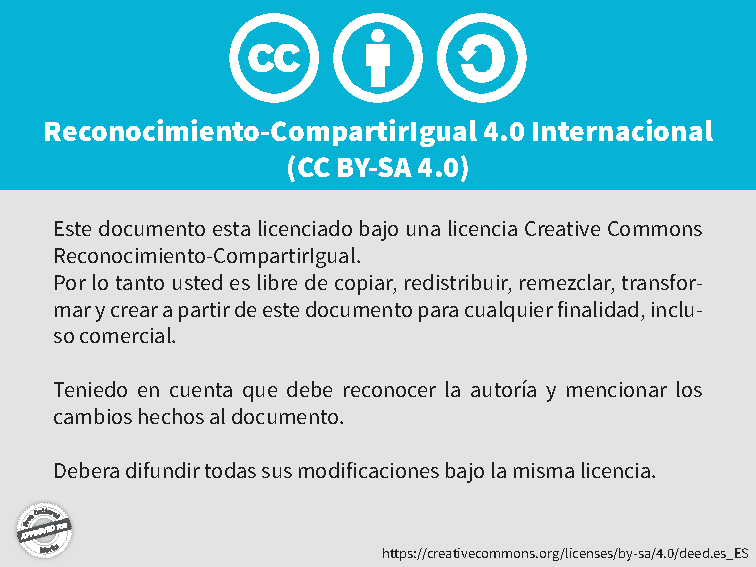
\includepdf[pages=1]{../Licencia_Diapositiva.pdf}}
\end{frame}
}

\section{Overleaf}
\begin{frame}{Overleaf}{}
\begin{center}
	
\includegraphics[width=0.7\linewidth]{Overleaf_Logo}
\end{center}

Página web: https://www.overleaf.com
\end{frame}

\begin{frame}{Overleaf}{}
\alert{\bf Overleaf} es una herramienta en línea de escritura de documentos en {\lmr\LaTeX} y texto enriquecido.\pause\\[1em]

Posee una gran cantidad de convenios con instituciones educativas y publicaciones.\pause\\[1em]

Posee un soporte muy amplio a la mayoría de paquetes y «sabores» de {\lmr\LaTeX}, con un editor que se puede personalizar a gusto, atajos de teclado estilo Emacs o Vim, y un visor integrado.
\end{frame}

\begin{frame}[plain]{}{}
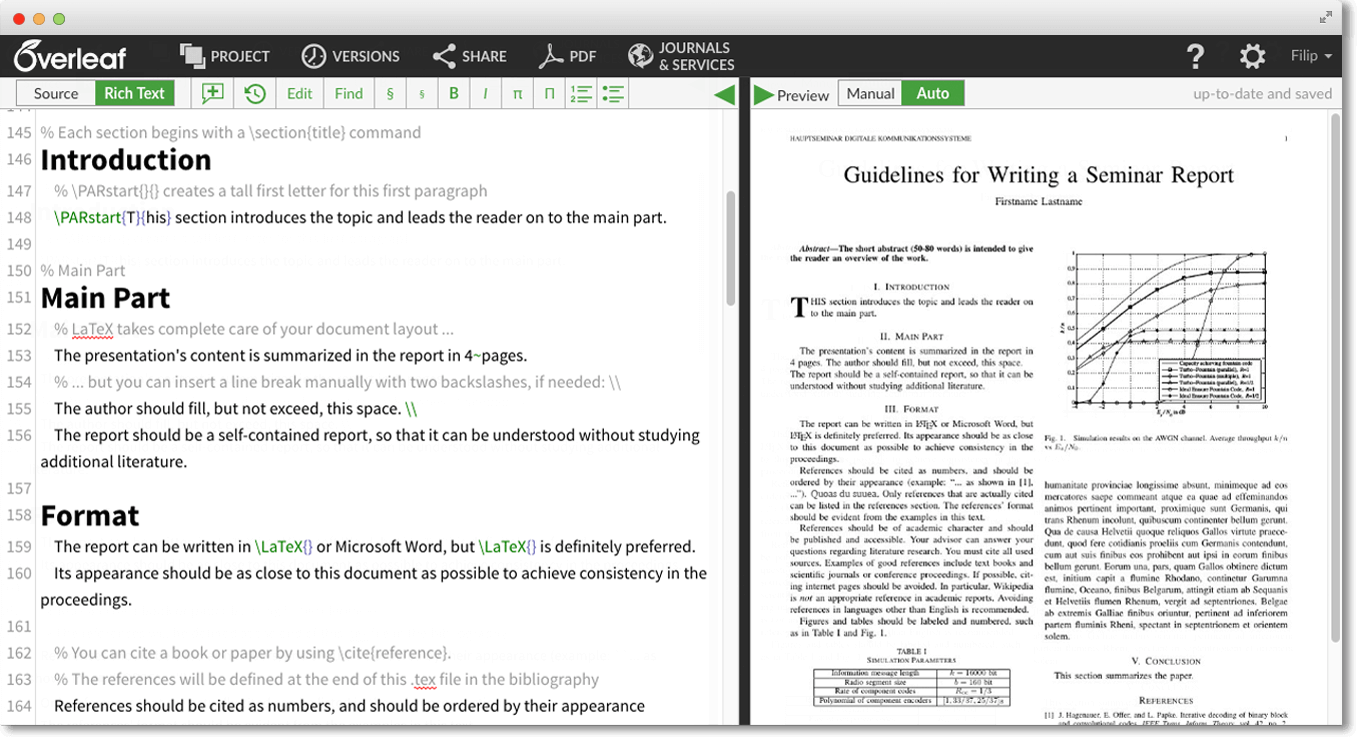
\includegraphics[width=\linewidth]{Overleaf_Screen}
\end{frame}

\section{ShareLaTeX}
\begin{frame}{ShareLaTeX}{}
\begin{center}
	
\includegraphics[width=0.7\linewidth]{ShareLaTeX_Logo}
\end{center}

Página web: https://www.sharelatex.com
\end{frame}

\begin{frame}{ShareLaTeX}{}
\alert{\bf ShareLaTeX} es un editor de {\lmr\LaTeX} diseñado para ser ligero, rápido y sencillo.\pause\\[1em]

Tiene un amplio soporte a la mayoría de paquetes y «sabores» de {\lmr\LaTeX} al igual que Overleaf.\pause\\[1em]

También se puede personalizar su editor y los atajos de teclado, posee también un visor integrado.
\end{frame}

\begin{frame}[plain]{}{}
\centering
\ifratio
	{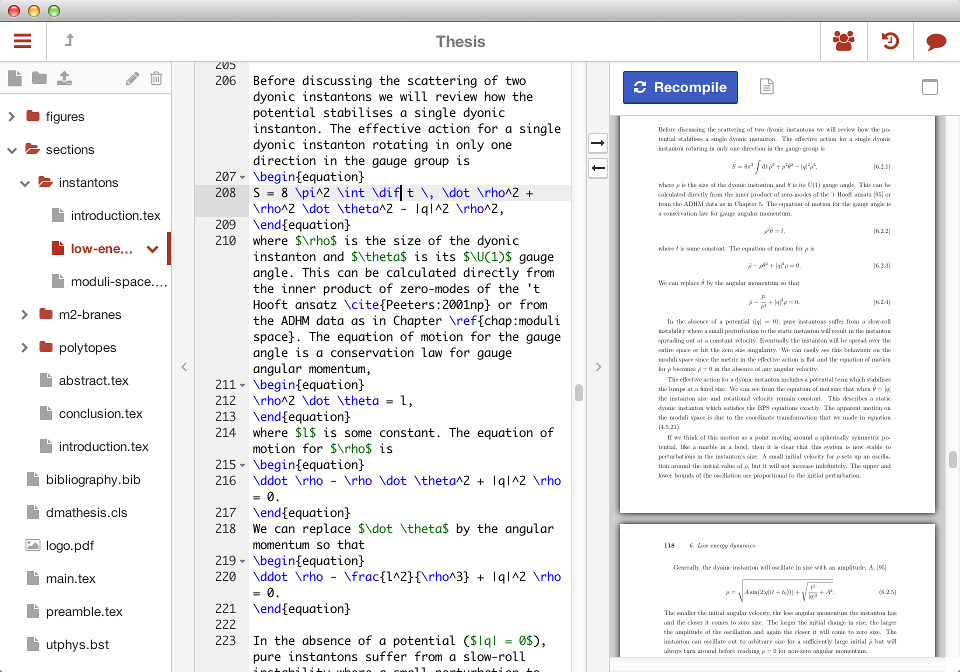
\includegraphics[width=0.8\linewidth]{ShareLaTeX_Screen}}
	{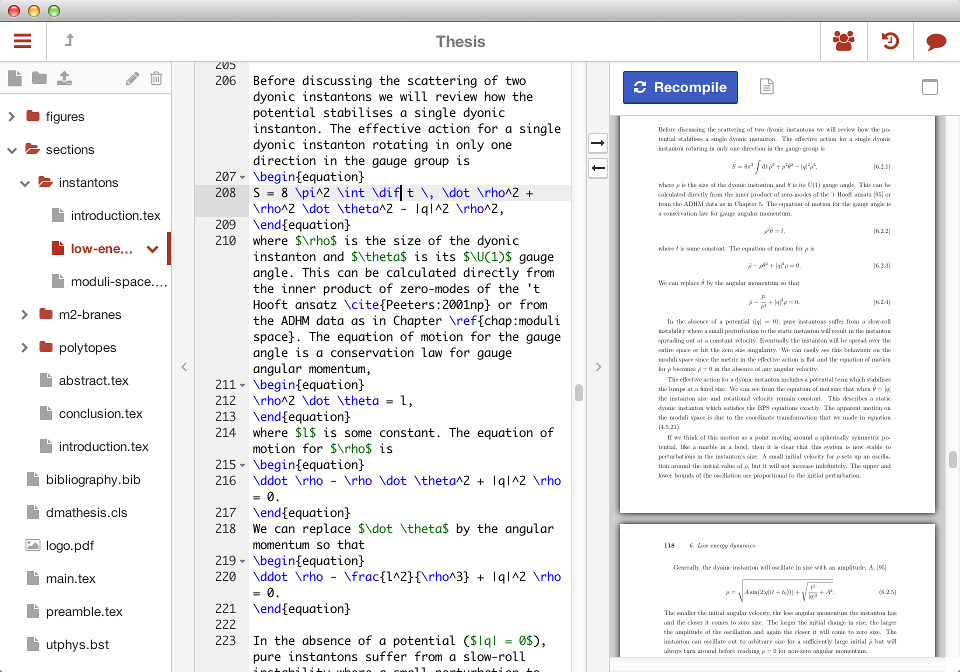
\includegraphics[width=\linewidth]{ShareLaTeX_Screen}}
\end{frame}

\section{Overleaf V2 (Overleaf+ShareLaTeX)}
\begin{frame}{Overleaf V2 (Overleaf+ShareLaTeX)}{}
\begin{center}
	
\includegraphics[width=0.7\linewidth]{Overleaf+ShareLaTeX_Logo}
\end{center}

Página web: https://v2.overleaf.com
\end{frame}

\begin{frame}{Overleaf V2 (Overleaf+ShareLaTeX)}{}
\alert{\bf Overleaf V2} es un editor creado por la unión de Overleaf y ShareLaTeX.\pause\\[1em]

De forma que se unen todas las características de estos dos editores. Obteniendo así un entorno de trabajo bastante agradable.\pause\\[1em]

Aunque se encuentra aún en desarrollo beta, es posible utilizar esta versión en la página web.
\end{frame}

\begin{frame}[plain]{}{}
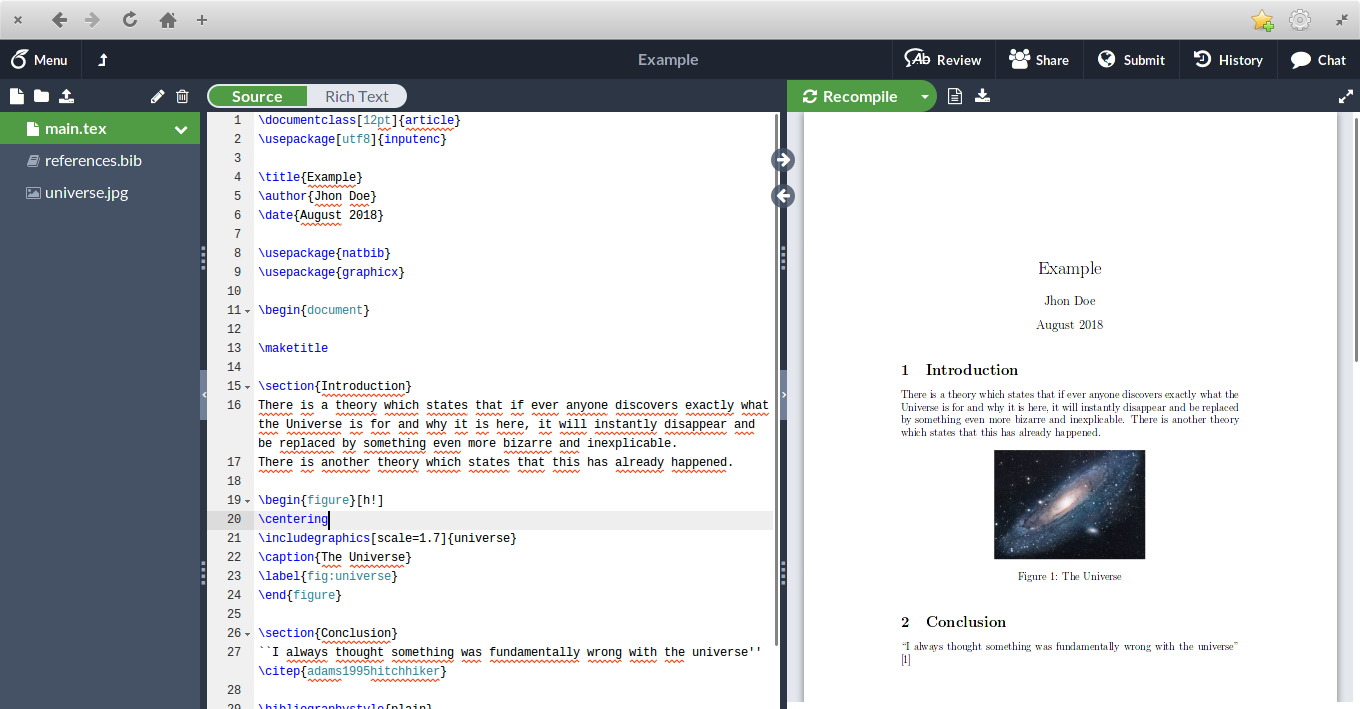
\includegraphics[width=\linewidth]{OverleafV2_Screen}
\end{frame}

\section{Papeeria}
\begin{frame}{Papeeria}{}
\begin{center}
	
\includegraphics[width=0.7\linewidth]{Papeeria_Logo}
\end{center}

Página web: https://www.papeeria.com
\end{frame}

\begin{frame}{Papeeria}{}
\alert{\bf Papeeria} es un editor mixto de Markdown y LaTeX.\pause\\[1em]

Funciona de manera similar a los otros editores, es muy simple y posee un amplio soporte a la mayoria de paquetes de {\lmr\LaTeX}.\pause\\[1em]

Funciona con {\lmr\TeX} Live 2015 - 2016. Lo que hace que sea un poco desactualizado para las versiones actuales de {\lmr\LaTeX}
\end{frame}

\begin{frame}[plain]{}{}
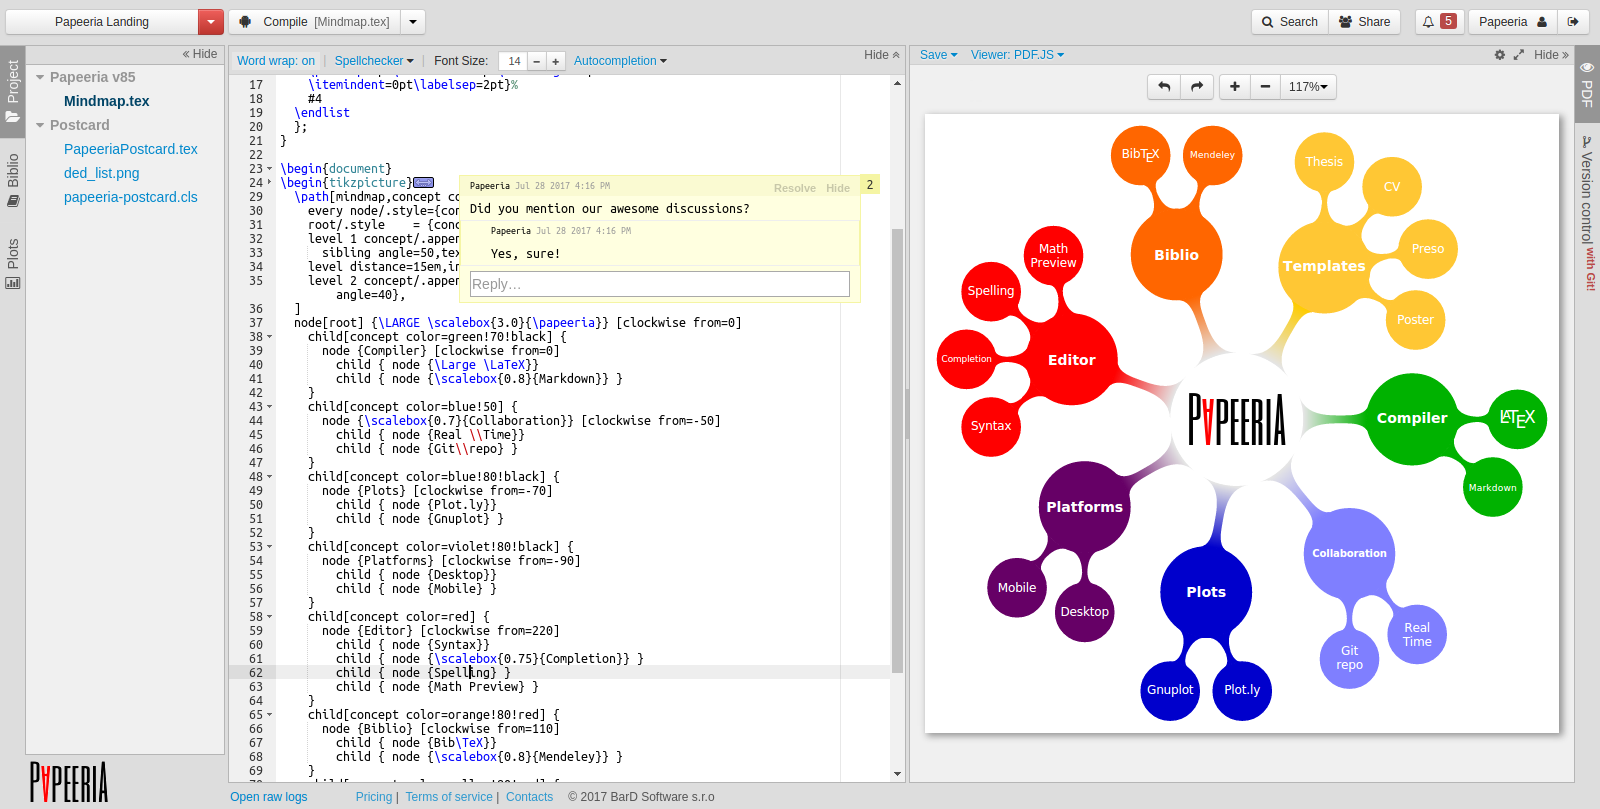
\includegraphics[width=\linewidth]{Papeeria_Screen}
\end{frame}

\section{LaTeX base}
\begin{frame}{LaTeX Base}{}
\begin{center}
	
\includegraphics[width=0.7\linewidth]{LaTeXBase_Logo}
\end{center}

Página web: https://www.latexbase.com
\end{frame}

\begin{frame}{LaTeX Base}{}
\alert{\bf LaTeX Base} es un editor muy enfocado en la colaboración y en la edición sin conexión.\pause\\[1em]

Aunque suene raro, LaTeX Base funciona sin conexión, pre-cargando la página, lo que hace que todo lo que estamos usando se cargue en el caché de nuestro ordenador y se pueda utilizar.\pause\\[1em]

Posee también un gran soporte a la mayoría de paquetes y «sabores» de {\lmr\LaTeX}, y un chat de voz para hacer más fácil la colaboración en tiempo real.
\end{frame}

\begin{frame}[plain]{}{}
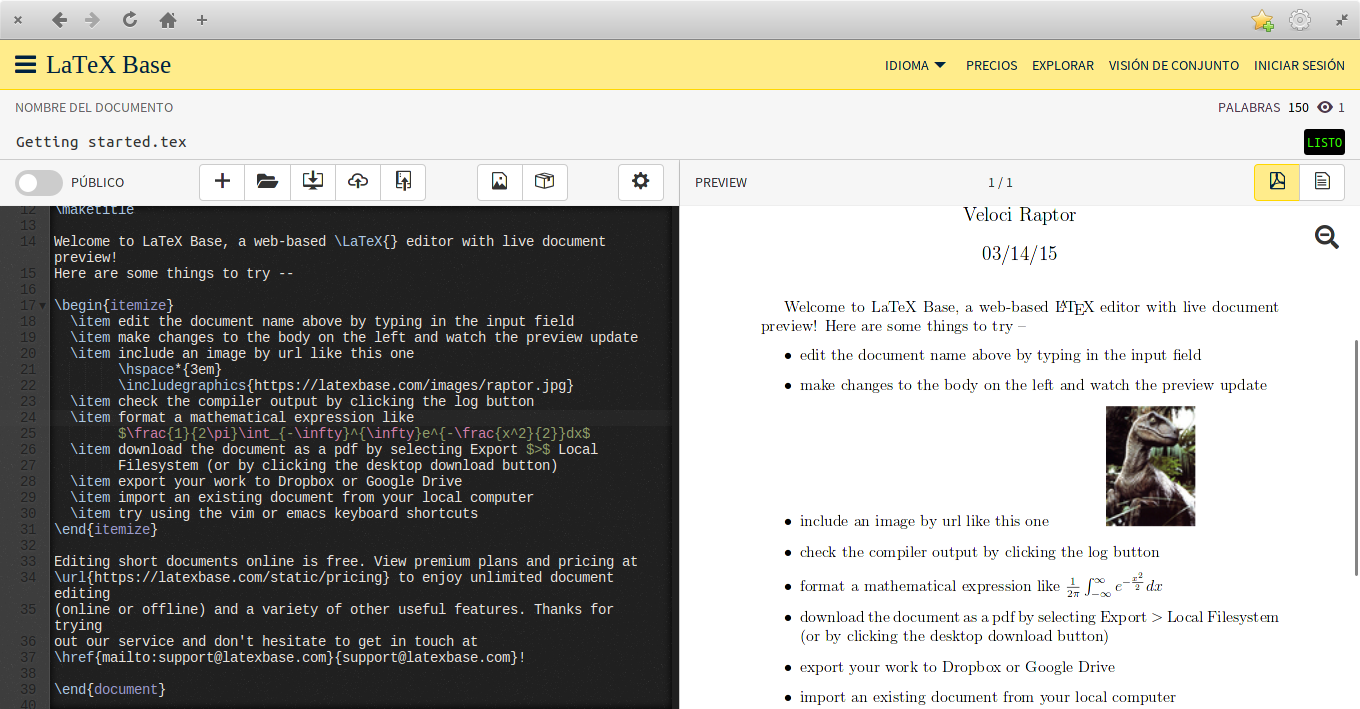
\includegraphics[width=\linewidth]{LaTeXBase_Screen}
\end{frame}

\section{Github y git}
\end{document}
